\documentclass{article}

\usepackage{fancyhdr}
\usepackage{extramarks}
\usepackage{amsmath}
\usepackage{amsthm}
\usepackage{amsfonts}
\usepackage{tikz}
\usepackage[plain]{algorithm}
\usepackage{algpseudocode}

\usetikzlibrary{automata,positioning}

%
% Basic Document Settings
%

\topmargin=-0.45in
\evensidemargin=0in
\oddsidemargin=0in
\textwidth=6.5in
\textheight=9.0in
\headsep=0.25in

\linespread{1.1}

\pagestyle{fancy}
\lhead{\hmwkAuthorName}
\chead{\hmwkClass\ (\hmwkClassInstructor\ \hmwkClassTime): \hmwkTitle}
\rhead{\firstxmark}
\lfoot{\lastxmark}
\cfoot{\thepage}

\renewcommand\headrulewidth{0.4pt}
\renewcommand\footrulewidth{0.4pt}

\setlength\parindent{0pt}

%
% Create Problem Sections
%

\newcommand{\enterProblemHeader}[1]{
    \nobreak\extramarks{}{Problem \arabic{#1} continued on next page\ldots}\nobreak{}
    \nobreak\extramarks{Problem \arabic{#1} (continued)}{Problem \arabic{#1} continued on next page\ldots}\nobreak{}
}

\newcommand{\exitProblemHeader}[1]{
    \nobreak\extramarks{Problem \arabic{#1} (continued)}{Problem \arabic{#1} continued on next page\ldots}\nobreak{}
    \stepcounter{#1}
    \nobreak\extramarks{Problem \arabic{#1}}{}\nobreak{}
}

\setcounter{secnumdepth}{0}
\newcounter{partCounter}
\newcounter{homeworkProblemCounter}
\setcounter{homeworkProblemCounter}{1}
\nobreak\extramarks{Problem \arabic{homeworkProblemCounter}}{}\nobreak{}

%
% Homework Problem Environment
%
% This environment takes an optional argument. When given, it will adjust the
% problem counter. This is useful for when the problems given for your
% assignment aren't sequential. See the last 3 problems of this template for an
% example.
%
\newenvironment{homeworkProblem}[1][-1]{
    \ifnum#1>0
        \setcounter{homeworkProblemCounter}{#1}
    \fi
    \section{Problem \arabic{homeworkProblemCounter}}
    \setcounter{partCounter}{1}
    \enterProblemHeader{homeworkProblemCounter}
}{
    \exitProblemHeader{homeworkProblemCounter}
}

%
% Homework Details
%   - Title
%   - Due date
%   - Class
%   - Section/Time
%   - Instructor
%   - Author
%

\newcommand{\hmwkTitle}{Homework\ \#1}
\newcommand{\hmwkDueDate}{September 2nd, 2014}
\newcommand{\hmwkClass}{Differential Equation}
\newcommand{\hmwkClassTime}{Section 061}
\newcommand{\hmwkClassInstructor}{Professor Heather Lee}
\newcommand{\hmwkAuthorName}{Yao Xiao}

%
% Title Page
%

\title{
    \vspace{2in}
    \textmd{\textbf{\hmwkClass:\ \hmwkTitle}}\\
    \normalsize\vspace{0.1in}\small{Due\ on\ \hmwkDueDate\ at 3:10pm}\\
    \vspace{0.1in}\large{\textit{\hmwkClassInstructor\ \hmwkClassTime}}
    \vspace{3in}
}

\author{\textbf{\hmwkAuthorName}}
\date{}

\renewcommand{\part}[1]{\textbf{\large Part \Alph{partCounter}}\stepcounter{partCounter}\\}

%
% Various Helper Commands
%

% Useful for algorithms
\newcommand{\alg}[1]{\textsc{\bfseries \footnotesize #1}}

% For derivatives
\newcommand{\deriv}[1]{\frac{\mathrm{d}}{\mathrm{d}x} (#1)}

% For partial derivatives
\newcommand{\pderiv}[2]{\frac{\partial}{\partial #1} (#2)}

% Integral dx
\newcommand{\dx}{\mathrm{d}x}

% Alias for the Solution section header
\newcommand{\solution}{\textbf{\large Solution}}

% Probability commands: Expectation, Variance, Covariance, Bias
\newcommand{\E}{\mathrm{E}}
\newcommand{\Var}{\mathrm{Var}}
\newcommand{\Cov}{\mathrm{Cov}}
\newcommand{\Bias}{\mathrm{Bias}}

\begin{document}

\maketitle

\pagebreak

\begin{homeworkProblem}
Draw a direction field for the given differential equation. Based on the direction field, determine the behavior of y as t \(\to\infty\). If this behavior depends on the initial value of y at t = 0, describe the dependency.

\textbf{Solution}
2. \(y'=2y-3\) \\
%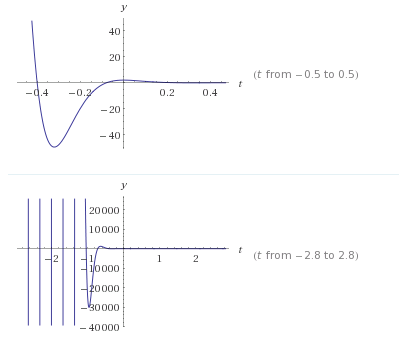
\includegraphics[scale=0.7]{images/prob1.png}  \\
when \(t\to\infty\)  the slope stays as -3 \\

5. \(y' =1+2y\) \\
%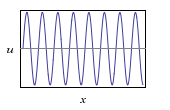
\includegraphics[scale=0.7]{images/prob2.png}  \\
when \(t\to\infty\)  the slope stays as 1 \\




\end{homeworkProblem}

\pagebreak

\begin{homeworkProblem}
Verify that each given function is a solution of the differ- ential equation.\\
8. \(y''+2y'-3y=0; y_1(t)=e^{-3t}; y_2(t)=e^t \) \\
\textbf{Solution}

For y1: \\
\[
    \begin{split}
	y1'(t) &= -3e^{-3t} 
	\\
	y1''(t) &= 9e^{-3t} 
	\\
	9e^{-3t}+2(-3e^{-3t})-3e^{3t} &= 9-6-3e^{3t} \\
	& = 0e^{-3t} \\
	& =0	
	\end{split}
\]
For y2: \\
\[
    \begin{split}
	y2'(t) &= e^{t} 
	\\
	y2''(t) &= e^{t} 
	\\
	e^{t}+2e^{t}-3e^{t} &= 0
	\end{split}
\]

So both of the solution are legit.

11. \(2t^2y''+3ty'-y=0 t>0 y_1(t)=t^{1/2} y_2(t)=t^{-1} \) \\

\[
    \begin{split}
	y1'(t) &= \frac{1}{2\sqrt{t}}
	\\
	y1''(t) &= \frac{-1}{(4 t^{3/2})}
	\\
	2t^2*\frac{-1}{(4 t^{3/2})}+3t*\frac{1}{2\sqrt{t}}-t^{1/2} &= -1/2 \sqrt{t} + 2/3 \sqrt{t} - \sqrt{t} \\
	&= 0
	\end{split}
\]

\[
    \begin{split}
	y2'(t) &= \frac{-1}{t^2}
	\\
	y2''(t) &= \frac{2}{t^{3}}
	\\
	\frac{2t^2*2}{t^3} - 3t*t^{-2}-t^{-1} &= 4/t-3/t-1/t \\
	&=0 \\
	\end{split}
\]

So both solutions are legit



\end{homeworkProblem}

\pagebreak

\begin{homeworkProblem}
\[
	\begin{split}
	y' = A(e^{-2t}(1-2t))\\
	2A(e^{-2t}(1-2t))+4Ate^{-2t}&=3e^{-2t}	\\ 
	LHS&=2Ae^{-2t}-4Ate^{-2t}+4Ate^{-2t}=2Ae^{-2t}\\
	&= 3e^{-2t}
	 A=1.5 \\
	\end{split}
	\]
	So A=1.5
\[
	\begin{split}
	y' &= Be^{-2t}\\
	2*-2Be^{-2t}+4Be^{-2t}&=3e^{-2t}	\\ 
	0 &= 3e^{-2t}
	\end{split}
	\]
	So there is no solution for this
\end{homeworkProblem}
\end{document}
